\documentclass[11pt]{article}
\usepackage[margin=2.2cm]{geometry}
\usepackage{amsmath,amssymb,booktabs,enumitem,graphicx}
\usepackage[hidelinks]{hyperref}
\setlist{nosep,leftmargin=*}
\setlength{\parindent}{0pt}

\newcommand{\dt}{\tilde\delta}
\newcommand{\nb}{\bar n}
\newcommand{\rmin}{r_{\min}(\nb)}

\title{02 --- Simulation: families, prior, constraints}
\date{17 September 2026}

\begin{document}
\maketitle

%==============================================================================
\section{Theory}

\subsection*{Aim}
\begin{itemize}
  \item Generate pool of patterns swept over the regime coordinates $(\nb, \dt)$; train and test are partitioned from it later
  \item Same $(\nb,\dt)$ distribution in every structured family, so regimes carry no info about the family
  \item Mat\'ern II: swept on $\dt$ like the rest, but its regimes are reported in $\mu_R$ (hard core in pairs, 01), since $\dt$ misses hard cores below $\rmin$
  \item Two patterns per $\theta$ so we can compute bias/variance at fixed $\theta$
\end{itemize}

\subsection*{Families}
Each $\theta$ = $\nb$ + \emph{shape} (drawn) + \emph{amplitude} (solved for the target $\dt$).

\smallskip
{\small
\begin{tabular}{@{}llll@{}}
\toprule
Family & Model & Shape & Amplitude \\
\midrule
Poisson & homogeneous, intensity $\nb$ & --- & --- \\
Thomas & parents $\kappa$; Poisson($\mu$) offspring, $N(0,\sigma^2 I)$; $\nb=\kappa\mu$ & $\sigma$ & $\mu$ \\
Nested & meta-parents $\kappa$; Poisson($\mu_1$) parents, $N(0,\sigma_1^2 I)$; & $\sigma_2$, $\rho=\sigma_1/\sigma_2$, $\mu_1$ & $\mu_2$ \\
 & \quad Poisson($\mu_2$) children, $N(0,\sigma_2^2 I)$; $\nb=\kappa\mu_1\mu_2$ & & \\
LGCP & $\Lambda = e^{\mu+Y}$, $\mathrm{Cov}\,Y = \sigma^2 e^{-r/s}$; $\nb = e^{\mu+\sigma^2/2}$ & $s$ & $\sigma^2$ \\
Mat\'ern II & primaries $\lambda_p$, hard core $R$ (type II); & --- & $R$ \\
 & \quad $\nb = (1-e^{-\lambda_p\pi R^2})/(\pi R^2)$ & & \\
\bottomrule
\end{tabular}}

\subsection*{Shape and amplitude}
\begin{itemize}
  \item Shape = where the structure lives (its length scale); amplitude = how strong it is at that scale
  \item At fixed $(\nb,\text{shape})$, amplitude $\to 0$ gives CSR; raising it strengthens the structure without moving it:
  \begin{itemize}
    \item Thomas $\mu$: same $\nb$ in fewer, bigger clusters ($\kappa=\nb/\mu$); nested $\mu_2$: same at the inner level
    \item LGCP $\sigma^2$: more variable intensity; Mat\'ern $R$: bigger hard core
  \end{itemize}
  \item $\dt$ increases monotonically with the amplitude (checked on grids), so each target $\dt$ has exactly one amplitude; solved by root-finding on the closed-form $K$ (\texttt{families.py})
\end{itemize}

\subsection*{Validity rules}
Each rule removes $\theta$ for which $\dt$ would be misleading. Rules 1--2 restrict the shape (a box of allowed shapes at each $\nb$); rules 3--4 cap the amplitude. Two tolerances: $\varepsilon = 0.2$, $c = 0.45$. Radius set $R(\nb)=[\rmin, 0.25]$ as in 01.
\begin{enumerate}
  \item \textbf{Scale inside $R(\nb)$} (shape)
  \begin{itemize}
    \item Why: $\dt$ only looks at $R(\nb)$. Structure mostly below $\rmin$ or beyond $0.25$ is missed, so patterns with the same $\dt$ would not be equally hard
    \item Rule: $\gamma(r)\in[0,1]$ = how much of the structure is still to come at $r$ (Thomas: $e^{-r^2/4\sigma^2}$, fraction of cluster pairs farther apart than $r$; LGCP: $e^{-r/s}$). Need $\gamma(\rmin)\ge\varepsilon$ and $\gamma(0.25)\le\varepsilon$
    \item Gives: $\sigma\in[\rmin,\,0.25]\,/\,2\sqrt{\ln(1/\varepsilon)}$ ($\sigma\le 0.098$); $s\in[\rmin,\,0.25]\,/\ln(1/\varepsilon)$ ($s \le 0.155$); nested: inner $\sigma_2$ for the lower bound, outer $\sqrt{\sigma_1^2+\sigma_2^2}$ for the upper
  \end{itemize}
  \item \textbf{Nested levels distinguishable} (shape)
  \begin{itemize}
    \item Why: otherwise nested is just a Thomas process
    \item Separated: inner level done ($\gamma_{\text{in}}\le\varepsilon$) before the outer one starts ($\gamma_{\text{out}}\ge1-\varepsilon$) $\Rightarrow$ $1+\rho^2\ge\ln(1/\varepsilon)/(-\ln(1-\varepsilon))$, i.e.\ $\rho\ge 2.49$
    \item Balanced: inner level carries at least $\varepsilon$ of the $K$ excess, $1/(1+\mu_1)\ge\varepsilon$ $\Rightarrow$ $\mu_1\le 4$; also $\mu_1\ge1$ (interpretability)
  \end{itemize}
  \item \textbf{Enough independent units} (amplitude)
  \begin{itemize}
    \item Why: $\dt$ is computed at $\nb$, so it only means something if $n\approx\nb$. Few big clusters make $n$ swing
    \item Rule: $\mathrm{CV}(n)=\mathrm{sd}(n)/\nb \le c$, with
    \[
      \mathrm{CV}^2 = \frac1{\nb} + \int_0^1 \bar\gamma_W(r)\, \mathrm d\big(K(r)-\pi r^2\big),
      \qquad \bar\gamma_W(r) = 1-\tfrac{4r}{\pi}+\tfrac{r^2}{\pi} \ \text{(isotropised set covariogram of $W$)}
    \]
    \item Formula vs simulated Thomas CV: 0.409/0.413, 0.310/0.306, 0.444/0.445
    \item Old DV3 in these terms: Thomas 0.41--0.44, nested 0.26--0.31, LGCP up to 0.72 (inconsistent)
  \end{itemize}
  \item \textbf{Mat\'ern II packing} (amplitude)
  \begin{itemize}
    \item Why: type II thinning cannot pass fill $\pi R^2\nb = 1$; near it the process degenerates
    \item Rule: $\pi R^2\nb \le 0.95$ ($\lambda_p \le 3.15\,\nb$)
  \end{itemize}
\end{enumerate}
With $\varepsilon=0.2$ we recover the old DV3 bounds ($\sigma\le0.1$, $s\le0.15$, $\rho\ge3$); only the LGCP lower bound on $s$ is wider (0.5 $\to$ 0.16--0.055 spacings).

\subsection*{Feasibility and the $\dt$ range}
Largest $\dt$ reachable under the rules (\texttt{scripts/feasibility.py}):

\smallskip
\begin{tabular}{@{}lrrrrrr@{}}
\toprule
$\nb$ & 100 & 152 & 230 & 348 & 528 & 800 \\
\midrule
Thomas & 16.8 & 26.9 & 42.3 & 65.5 & 101 & 155 \\
Nested & 14.4 & 23.9 & 38.7 & 61.7 & 97.1 & 150 \\
LGCP & 17.3 & 27.4 & 42.3 & 63.9 & 95.6 & 148 \\
Mat\'ern II & 4.3 & 5.3 & 6.5 & 8.0 & 9.9 & 11.9 \\
\bottomrule
\end{tabular}
\begin{itemize}
  \item Cluster families $\propto\nb$ (CV fixes the clustering, $s_0\propto 1/n$); Mat\'ern $\propto\sqrt{\nb}$ (packing limit)
  \item Mat\'ern cap physical: fill 0.95 $\to$ 0.999 moves it 4.34 $\to$ 4.45 at $\nb=100$
  \item Common range at every $\nb$ $\Rightarrow$ $\dt\in[\delta_{lo}, 4]$; $\nb$ and $\dt$ independent
  \item $\delta_{lo}=0.1$ for now; any larger $\delta_{lo}$ is a subset of this pool (log-uniform restricts to log-uniform)
\end{itemize}

\subsection*{Prior (draw order is part of the definition)}
\begin{enumerate}
  \item $\nb \sim$ log-uniform$[100, 800]$
  \item $\dt \sim$ log-uniform$[0.1, 4]$ (Poisson: $\dt = 0$, skip 2--4)
  \item Shape: each coordinate log-uniform on its rule-1/2 box at $\nb$; redraw until valid, $\dt$ reachable, and (LGCP) a grid exists
  \item Amplitude: the unique $a$ with $\dt(\nb,\text{shape},a) = $ target (root in $\log a$), must be below the rule-3/4 cap
\end{enumerate}
\begin{itemize}
  \item Amplitude is not drawn, so its distribution is whatever the $\dt$ prior induces (Fig.~\ref{fig:prior})
\end{itemize}

\subsection*{Samplers}
\begin{itemize}
  \item Poisson: $N\sim\mathrm{Poisson}(\nb)$ uniform points
  \item Thomas / nested: top-level parents on $W$ expanded by $5\times$ the total displacement s.d.\ (missed mass $e^{-12.5}$), offspring, crop to $W$
  \item Mat\'ern II: primaries on $W\oplus R$ with $U(0,1)$ marks, delete a point if a neighbour within $R$ has a smaller mark, crop (exact)
  \item LGCP: circulant embedding on the $(2M)^2$ torus, spacing $1/M$: $Y = \mathcal F^{-1}[\sqrt{\lambda}\,\mathcal F w]$, $w$ white noise, $\lambda = \mathcal F(\text{covariance})$ (exact on the grid); Poisson cell counts, uniform in cells
  \begin{itemize}
    \item $M$: smallest power of two $\ge128$ with $|K_{\text{grid}}-K|\le 0.1\cdot 2\pi r\, s_0(r;\nb)$ on $R(\nb)$
    \item Grid $K$: bilinear interpolation of $e^{C}$ on the lattice, midpoint rule at $1/(4M)$
  \end{itemize}
  \item Patterns conditioned on $n\in[20,2000]$ (tables' domain), redrawn from the same stream
\end{itemize}

%==============================================================================
\section{Implemented pipeline}

\subsection*{Code}
\begin{tabular}{@{}ll@{}}
\toprule
\texttt{src/cloudforger/simulation/seeding.py}   & addressed random streams \\
\texttt{src/cloudforger/simulation/families.py}  & rules, shape boxes, $K-\pi r^2$, CV, $\dt$, amplitude solve \\
\texttt{src/cloudforger/simulation/processes.py} & the five samplers \\
\texttt{src/cloudforger/simulation/lgcp\_grid.py} & LGCP grid size \\
\texttt{src/cloudforger/simulation/sweep.py}     & $\theta$ draw, replicate patterns, shards \\
\texttt{src/cloudforger/simulation/check.py}     & mean $\hat K$ vs closed form \\
\texttt{scripts/simulate.py}                     & CLI: \texttt{run}, \texttt{merge}, \texttt{check} \\
\texttt{scripts/feasibility.py}                  & maximum reachable $\dt$ \\
\texttt{scripts/simulation\_figures.py}          & figures of this document \\
\texttt{configs/simulation/config.yaml}          & $\nb$, $\dt$ range, rules, sizes \\
\bottomrule
\end{tabular}

\subsection*{Configuration}
\begin{itemize}
  \item 10\,000 $\theta$ per family $\times$ 2 patterns = 20\,000 patterns per family, 100\,000 total
  \item $\nb\in[100,800]$, $\dt\in[0.1,4]$, $\varepsilon=0.2$, $c=0.45$, fill 0.95, $\mu_1\ge1$; shards of 250 $\theta$
\end{itemize}

\subsection*{Seeding}
\begin{itemize}
  \item Key $(\text{DV}=3,\ \text{set},\ \text{family},\ \text{index},\ \text{role})$, root shared with 01
  \item $\theta$: (\texttt{sweep}, family, $i$, PARAMS); pattern: (\texttt{sweep}, family, $2i+\text{rep}$, PATTERN)
  \item Checks: (\texttt{pilot}, family, $10^9 + 10^4 i + p$); gallery (\texttt{pilot}, $2\cdot 10^9 + \dots$); both disjoint from the null curves of 01
  \item More $\theta$ later: append indices, nothing existing changes
\end{itemize}

\subsection*{Steps}
\begin{enumerate}
  \item \textbf{Run} (\texttt{run --jobs 10}; 3\,min 10\,s on 10 cores): one file per shard, atomic, resumable
  \item \textbf{Merge} (\texttt{merge}): per family \texttt{points.npz} (points, offsets) + \texttt{manifest.csv} in \texttt{data/simulation/}; $\sim$106\,MB each
  \begin{itemize}
    \item Manifest: \texttt{case\_id} (\texttt{family-theta-rep}), $\nb$, $\dt$, CV, amplitude, shape, model parameters, LGCP $M$, $n$, tries
  \end{itemize}
  \item \textbf{Check} (\texttt{check}): 8 $\theta$ per family, 500 patterns each; $\tilde K = \hat K\, n(n-1)/\nb^2$ (unbiased) vs closed form on 16 radii of $R(\nb)$
\end{enumerate}

\subsection*{Results}
{\small
\begin{tabular}{@{}lll@{}}
\toprule
Check & Result & Reference \\
\midrule
Closed-form $K$ vs old DV3 implementation & $\le 10^{-10}$ & --- \\
Sampler $\tilde K$ vs $K$, max $|z|$ & 1.6--2.8 by family & $\lesssim 3.4$ (16 radii) \\
Sampler $\tilde K$ vs $K$, max rel.\ error & $\le 3.2\%$; Mat\'ern 10\% at $K\approx0$ & --- \\
$\log\dt$ uniform, KS distance & $\le 0.0075$ & 0.0136 (1\%) \\
Shape draws per $\theta$ & 1; nested mean 1.96, max 14 & --- \\
Pattern redraws ($n\notin[20,2000]$) & 0; realised $n$ 44--961 & --- \\
Realised max CV & Thomas 0.32, nested 0.30, LGCP 0.34 & $c = 0.45$ \\
LGCP grid $M$ (128/256/512/1k/2k/4k) & 8064/1013/566/268/76/13 $\theta$ & --- \\
5\% L-test size, Poisson pool & 0.049 (20\,000 patterns) & 0.05 \\
\bottomrule
\end{tabular}}

%==============================================================================
\section{Regimes}

\begin{figure}[h]
\centering
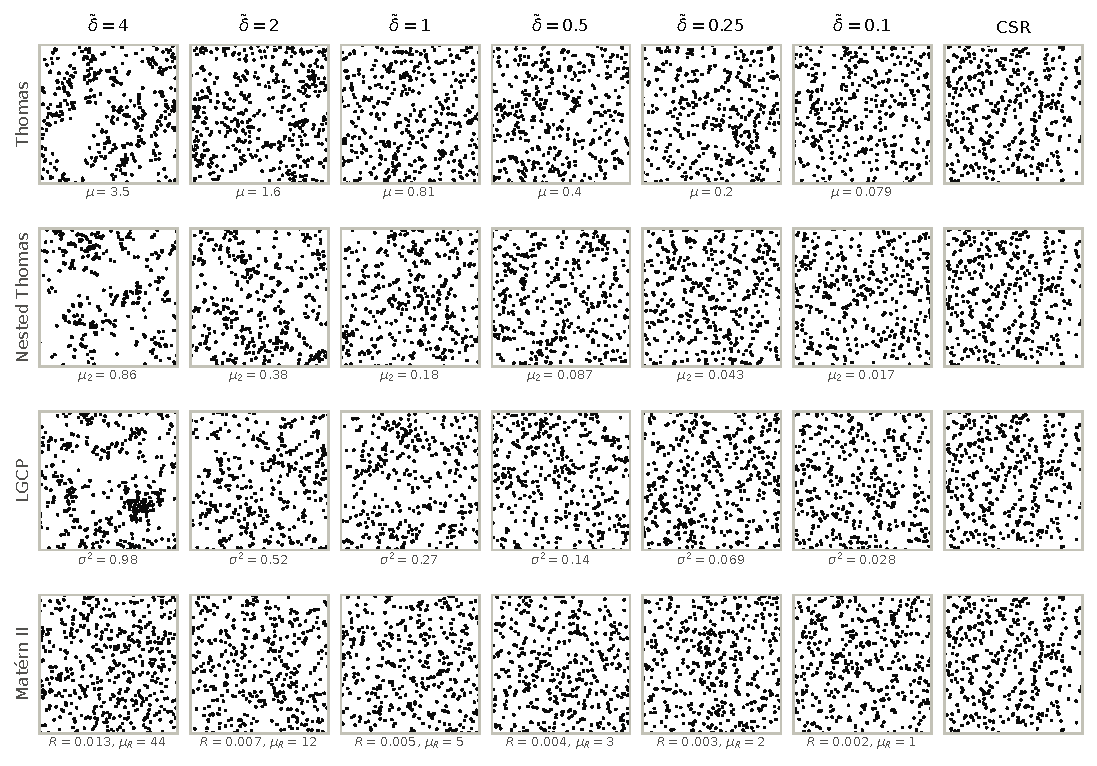
\includegraphics[width=\textwidth]{figs/02_regime_patterns.pdf}
\caption{One pattern per cell, $\nb=400$, fixed shape per family (Thomas $\sigma=0.03$; nested $\sigma_2=0.008$, $\rho=5$, $\mu_1=3$; LGCP $s=0.04$). Only the amplitude changes along a row.}
\label{fig:patterns}
\end{figure}

\begin{figure}[h]
\centering
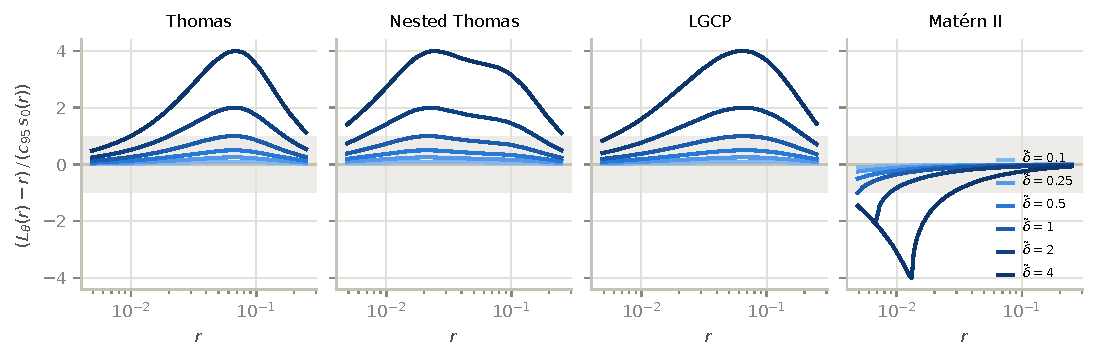
\includegraphics[width=\textwidth]{figs/02_regime_curves.pdf}
\caption{Closed-form $L_\theta(r)-r$ in units of the critical envelope, same $\theta$ as Fig.~\ref{fig:patterns}, on $R(400)$. Grey band: rejection boundary. Peak height $=\dt$.}
\label{fig:curves}
\end{figure}

\begin{figure}[h]
\centering
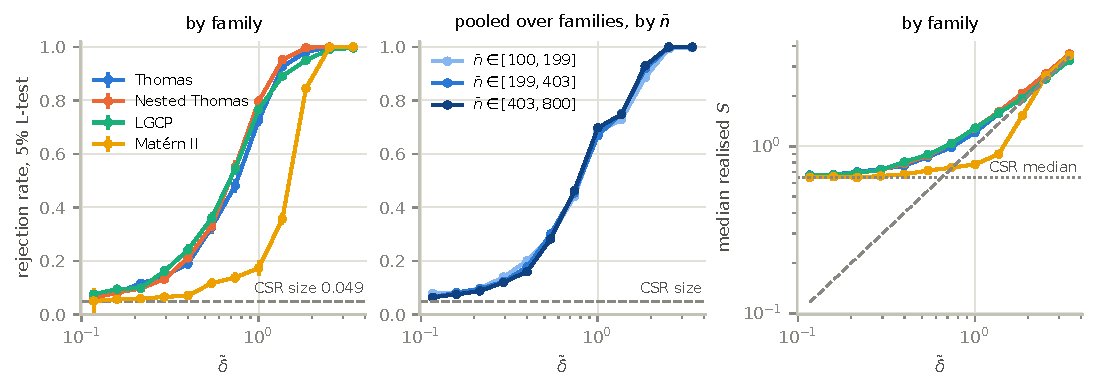
\includegraphics[width=\textwidth]{figs/02_power.pdf}
\caption{The 5\% L-test of 01 on all 100\,000 simulated patterns. Left: rejection rate by family, 12 log-bins of $\dt$, 95\% intervals. Middle: pooled over families, by $\nb$ tercile. Right: median realised $S$ (dashed: $S=\dt$; dotted: CSR median).}
\label{fig:power}
\end{figure}

\begin{figure}[h]
\centering
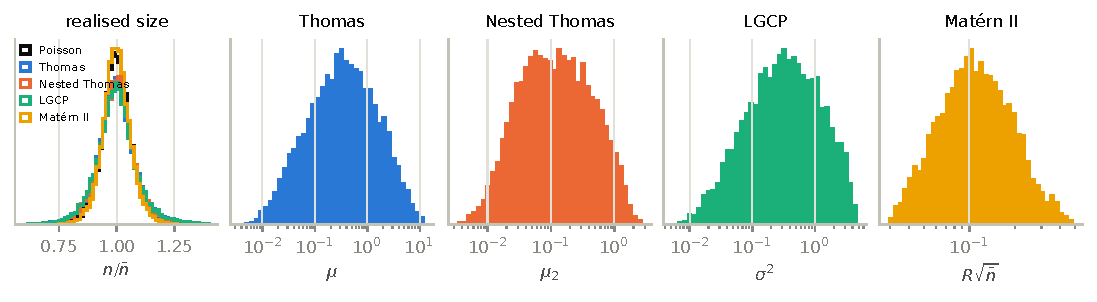
\includegraphics[width=\textwidth]{figs/02_prior.pdf}
\caption{Left: realised $n/\nb$. Right: induced distribution of the solved amplitude (Mat\'ern: $\tau=R\sqrt{\nb}$).}
\label{fig:prior}
\end{figure}

\clearpage
\subsection*{What the figures show}
\begin{itemize}
  \item \textbf{Convergence to Poisson} (Figs.~\ref{fig:patterns}, \ref{fig:curves}): along each row only the amplitude moves; curves shrink uniformly into the null band; at $\dt\le0.25$ patterns are visually CSR
  \item \textbf{Scale structure survives the amplitude}: nested keeps its two-step shoulder at every $\dt$; Mat\'ern's deficit sits just above $\rmin$
  \item \textbf{Same regime, same difficulty across families, for the $L$ test} (Fig.~\ref{fig:power}, left; Mat\'ern is much easier for a nearest-neighbour test, 01):
  \smallskip

  \begin{tabular}{@{}lrrrrrr@{}}
  \toprule
  $\dt$ bin & (0.1, 0.2] & (0.2, 0.4] & (0.4, 0.8] & (0.8, 1.25] & (1.25, 2] & (2, 4] \\
  \midrule
  Thomas & 0.078 & 0.136 & 0.339 & 0.712 & 0.952 & 0.999 \\
  Nested & 0.072 & 0.135 & 0.366 & 0.779 & 0.974 & 1.000 \\
  LGCP & 0.085 & 0.152 & 0.386 & 0.746 & 0.923 & 0.988 \\
  Mat\'ern II & 0.059 & 0.084 & 0.214 & 0.639 & 0.914 & 0.997 \\
  \bottomrule
  \end{tabular}
  \item \textbf{$\dt$ absorbs $\nb$} (middle): terciles $[100,199]$, $[199,403]$, $[403,800]$ agree within 0.03 in every bin
  \item \textbf{Floor and ceiling}: below $\dt\approx0.25$ rejection $\le 0.15$ and median $S$ = CSR median (0.65); above $\dt\approx1.25$ rejection $\ge 0.91$ and median $S\approx\dt$
  \item \textbf{Correction to 01}: at $\dt\approx1$ rejection is 0.64--0.78, not $\approx$50\%: pattern noise adds to the sup, so $S$ tends to exceed $\dt$
  \item \textbf{Replicates}: the two patterns of a $\theta$ agree on rejection 77--82\% of the time; correlation of $\log S$ 0.71--0.82
\end{itemize}

\subsection*{Coverage}
\textbf{$\dt$ coverage.} Cells: 6 log-$\dt$ bins $\times$ 3 log-$\nb$ bins, expected 556 $\theta$ each.

\smallskip
{\small
\begin{tabular}{@{}lrrrr@{}}
\toprule
Family & realised $\dt$ & $\log\dt$ uniform (KS $p$) & $\nb \perp \dt$ ($\chi^2$ $p$) & $\theta$ per cell \\
\midrule
Thomas & 0.1001--3.9998 & 0.76 & 0.81 & 530--581 \\
Nested & 0.1000--3.9969 & 0.98 & 0.54 & 519--587 \\
LGCP & 0.1000--3.9984 & 0.78 & 0.44 & 524--589 \\
Mat\'ern II & 0.1001--3.9939 & 0.60 & 0.43 & 514--601 \\
\bottomrule
\end{tabular}}

\medskip
\textbf{Parameter coverage at each $\dt$.} At fixed $(\nb,\dt)$ the allowed parameters are the shapes passing rules 1--2 at $\nb$; the amplitude is then determined.
\begin{itemize}
  \item \textbf{By construction}: shape drawn after $\dt$, from its own uniforms; replay of every $\theta$ with $\dt<0.2$ or $\dt>3$: 0 shapes rejected by the amplitude solve (only nested geometric rejections) $\Rightarrow$ at every $\dt\le4$ the shape distribution is the full rule-1/2 prior, independent of $\dt$
  \item \textbf{Range}: normalised position $u=\log(x/x_{lo})/\log(x_{hi}/x_{lo})$ in the box at $\nb$ spans 0.000--1.000 in every $\dt$ bin (Thomas $\sigma$, LGCP $s$, nested $\mu_1$); nested $\sigma_2$, $\rho$ reach 0.97--0.99 (top corner of the $(\sigma_2,\rho)$ region excluded by the outer-scale rule)
  \item \textbf{Uniformity}: Thomas, LGCP uniform in $u$ within each $\dt$ bin (KS $p$ 0.08--0.94); $u$-quintile $\perp$ $\dt$ bin ($\chi^2$ $p$ 0.10--0.81, all shape coordinates)
  \item \textbf{Nested}: vs a direct rejection sample of the allowed region at the same $\nb$: pooled KS $p$ 0.53--0.93; 3 of 18 per-bin tests $<0.05$ (multiple testing; excluded as bias by the replay)
  \item \textbf{Amplitude range at fixed $\dt$}: wide, because the amplitude compensates for $\nb$ and shape (e.g.\ larger $\nb$ needs a weaker structure for the same $\dt$). Realised ($\dt$ within $\pm10\%$) vs theory (grid over $\nb$ and allowed shapes):

  \smallskip
  {\footnotesize
  \begin{tabular}{@{}lllllll@{}}
  \toprule
   & \multicolumn{2}{c}{Thomas $\mu$} & \multicolumn{2}{c}{LGCP $\sigma^2$} & \multicolumn{2}{c}{Mat\'ern $R$} \\
  $\dt$ & realised & theory & realised & theory & realised & theory \\
  \midrule
  0.1 & 0.0037--0.32 & 0.0033--0.35 & 0.0055--0.28 & 0.0049--0.27 & 0.0010--0.0082 & 0.0010--0.0079 \\
  0.5 & 0.019--1.5 & 0.018--1.7 & 0.027--1.2 & 0.025--1.2 & 0.0022--0.017 & 0.0022--0.017 \\
  1 & 0.042--3.6 & 0.040--3.5 & 0.047--2.1 & 0.049--2.1 & 0.0029--0.022 & 0.0029--0.022 \\
  4 & 0.31--12 & 0.25--14 & 0.22--4.8 & 0.19--5.0 & 0.0059--0.047 & 0.0068--0.051 \\
  \bottomrule
  \end{tabular}}

  Theory grid coarse, so realised can exceed it
  \item \textbf{Density}: one-shape families $\ge$297 $\theta$ per ($\dt$ bin, shape quintile); nested $\ge$62 per ($\dt$ bin, marginal quintile), but jointly $\approx 10^4/(6\cdot5^3)\approx13$ per cell
\end{itemize}

%==============================================================================
\section{Statistical notes}

\subsection*{Interpretation}
\begin{itemize}
  \item Regimes defined by one classical yardstick ($L$); visually, Mat\'ern inhibition at $\dt\le4$ is hard to see by eye although the test sees it
  \begin{itemize}
    \item $\nb=400$, $\dt=4$: $R=0.0127$ (0.25 spacings), $\pi R^2\nb=0.20$; 25 fresh patterns all visually near-CSR, all with $S\in[3.76, 4.48]$; minimum pair distance $\ge R$ (sampler correct)
    \item Removes only pairs closer than a quarter spacing; visibly regular patterns need fill $\approx0.95$, i.e.\ $\dt\approx8.6$ at $\nb=400$ (outside the common range)
  \end{itemize}
  \item Mat\'ern lags in $(0.2, 1.25]$: for $\dt\lesssim1$ its hard core lies below $\rmin$, outside $R(\nb)$, so $\dt$ and the test see only the deficit's tail (01). A nearest-neighbour test detects the same patterns with power 0.63--1.00 $\Rightarrow$ equal $\dt$ means equal difficulty for the $L$ test only
  \item Shape distribution at every $\dt$ is the full rule-1/2 prior (Coverage): no shape rejected by the amplitude solve; nested redraws are geometric (the $\rho$--$\sigma_2$ coupling)
  \item Allowed shape box depends on $\nb$ (lower bound $\propto\rmin$): in absolute units the smallest scales occur only at large $\nb$; in normalised $u$, shape $\perp\nb$
  \item Mat\'ern II has no shape: $(\nb,\dt)$ determines $R$ $\Rightarrow$ regime-conditional inference error for Mat\'ern conditions on almost the whole parameter (within a $\dt$ bin $R$ still varies $\approx8\times$ via $\nb$ and bin width); not comparable one-to-one with families that keep shape variation
  \item Rule 3 inactive in this range (max realised CV 0.34 $< 0.45$): it matters only if $\dt$ is ever raised
  \item Induced amplitude marginals (Fig.~\ref{fig:prior}) are the effective inference prior: learned estimators shrink toward them
\end{itemize}

\subsection*{Scope and limits}
\begin{itemize}
  \item $\dt$ at $\nb$; realised $n/\nb$ 5--95\%: 0.89--1.11 (Poisson, Mat\'ern), 0.85--1.15 (clustered)
  \item Gallery and curves at one shape per family and $\nb=400$: illustrative, not exhaustive; the power table uses the whole pool
  \item LGCP: grid process, bias bounded at $0.1\,s_0$; exact circulant embedding on a $2\times$ torus
  \item Thomas/nested buffer truncation $e^{-12.5}$
\end{itemize}

\subsection*{Open}
\begin{itemize}
  \item $\delta_{lo}$: the classical test is at its floor below $\approx 0.25$; decide with learned methods' curves
  \item Carving train/validation/test from the pool (by $\theta$, both replicates together)
  \item Mat\'ern below $\mu_R\approx1$ (hard for every test) is not sampled: the $\dt$ floor 0.1 corresponds to $\mu_R\approx1$
  \item Nested joint shape coverage thin ($\approx$13 $\theta$ per $\dt$ bin $\times$ $5^3$ cell): enough for averaging over shape, not for joint shape analysis; more $\theta$ can be appended
  \item Shard files (\texttt{data/simulation/shards/}, 626\,MB) redundant after merge
\end{itemize}

\end{document}
